\documentclass{article} % For LaTeX2e
\usepackage{nips15submit_e,times}
\usepackage{graphicx}
%\usepackage{epsfig}
\usepackage{amsmath}
\usepackage{amssymb}
\usepackage[pagebackref=true,breaklinks=true,letterpaper=true,colorlinks,bookmarks=false]{hyperref}
\usepackage{url}
\usepackage[UTF8]{ctex}


\title{基于深度卷积神经网络的 ImageNet 分类}


\author{
Alex Krizhevsky\\
多伦多大学\\
\texttt{kriz@cs.utoronto.ca}\\
\And
Ilya Sutskever\\
多伦多大学\\
\texttt{ilya@cs.utoronto.ca}\\
\And
Geoffrey E. Hinton\\
多伦多大学\\
\texttt{hinton@cs.utoronto.ca}\\
%(if needed)\\
}

% The \author macro works with any number of authors. There are two commands
% used to separate the names and addresses of multiple authors: \And and \AND.
%
% Using \And between authors leaves it to \LaTeX{} to determine where to break
% the lines. Using \AND forces a linebreak at that point. So, if \LaTeX{}
% puts 3 of 4 authors names on the first line, and the last on the second
% line, try using \AND instead of \And before the third author name.

\newcommand{\fix}{\marginpar{FIX}}
\newcommand{\new}{\marginpar{NEW}}

\nipsfinalcopy % Uncomment for camera-ready version

\begin{document}

{\small
\maketitle
}
\renewenvironment{abstract}{\vskip.075in\centerline{\large\bfseries
摘要}\vspace{0.5ex}\begin{quote}}{\par\end{quote}\vskip 1ex}

\begin{abstract}

我们训练了一个大型的深度卷积神经网络, 将 ImageNet LSVRC-2010 竞赛中的 120 万张高分辨率图片分类到 1000 个不同类别. 在测试数据上, 我们达到了 37.5\% 和 17.0\% 的 top-1 和 top-5 错误率, 这比之前的最新技术要好的多. 该神经网络有 6000 万个参数和 650,000 个神经元, 由 5 个卷积层, 其中一些后面跟着最大池化层, 以及 3 个全连接层, 和最后一个 1000 路 softmax 组成. 为了让训练更快, 我们使用了非饱和神经元和卷积操作的一个非常高效的 GPU 实现. 为了减少全连接层中的过拟合, 我们采用了一个最近开发的称为“dropout”的正则化方法, 该方法被证明非常有效. 我们还在 ILSVRC-2012 竞赛中使用这个模型的一个变体, 获得了 15.3\% 的 top-5 测试错误率, 而第二名为 26.2\%.
\end{abstract}
\vspace{-2ex}

\section{引言}
\vspace{-2ex}

当前的对象识别方法主要依赖机器学习方法. 为了提高其性能, 我们可以收集更大的数据集, 学习更强大的模型, 并使用更好的技术来防止过拟合. 直到最近, 标记图像的数据集相对较小——通常只有几万张图像 (例如, NORB~\cite{lecun2004}、Caltech-101/256~\cite{feifei2007, griffin2007} 和 CIFAR-10/100~\cite{krizhevsky2009}). 简单的识别任务可以使用这种大小的数据集很好地解决, 尤其是如果它们使用保持标签的转换进行增强. 例如, MNIST 数字识别任务的当前最佳错误率 (\textless 0.3\%) 接近人类表现~\cite{cire2012}. 但是现实环境中的物体表现出相当大的可变性, 因此要学会识别它们, 有必要使用更大的训练集. 事实上, 小型图像数据集的缺点已被广泛认可 (例如, Pinto 等人~\cite{pinto2008}), 但直到最近才有可能收集具有数百万张图像的标记数据集. 新的更大数据集包括 LabelMe~\cite{russell2008}, 它由数十万张完全分割的图像组成, 以及 ImageNet~\cite{deng2009}, 它由超过 22, 000 个类别的超过 1500 万张标记的高分辨率图像组成.

要从数百万张图像中学习数千个对象, 我们需要一个具有更大学习能力的模型. 然而, 对象识别任务的巨大复杂性意味着即使像 ImageNet 这样大的数据集也无法指定这个问题, 因此我们的模型还应该有大量的先验知识来弥补我们没有的数据. 卷积神经网络 (CNN) 构成了这样一类模型~\cite{lecun2004, jarrett2009, krizhevsky2010, lee2009, lecun1990, pinto2009, turaga2010}. 它们的容量可以通过改变它们的深度和宽度来控制, 它们还对图像的性质做出了强有力的、大多正确的假设 (即统计数据的平稳性和像素依赖的局部性). 因此, 与具有类似大小的层的标准前馈神经网络相比, CNN 具有更少的连接和参数, 因此更容易训练, 而它们的理论上最佳性能可能只会略有下降.

尽管 CNN 具有很强的吸引力, 并且它们的局部架构相对高效, 但它们应用于大规模高分辨率图像时仍然过于昂贵. 幸运的是, 当前的 GPU 搭配 2D 卷积的高度优化实现, 足以促进有趣的大型 CNN 的训练, 而最近的数据集如 ImageNet 包含足够的标记示例来训练这些模型而不会严重过拟合.

本文的具体贡献如下: 我们在 ImageNet 的子集上训练了迄今为止最大的卷积神经网络, 该子集用于 ILSVRC-2010 和 ILSVRC-2012 竞赛, 并取得了这些数据集上有史以来最好的结果. 我们编写了一个高度优化的 GPU 实现 2D 卷积和所有其他在训练卷积神经网络中固有的操作, 并将其公开发布~\footnote{\url{http://code.google.com/p/cuda-convnet/}}. 我们的网络包含一些新的和不寻常的特性, 这些特性可以提高其性能并减少其训练时间, 详细信息在第~\ref{sec:arch} 节中说明. 我们的网络的大小使得过拟合成为一个严重的问题, 即使有 120 万个标记的训练示例, 所以我们使用了几种有效的防止过拟合的方法, 这些方法在第~\ref{sec:overfit} 节中描述. 我们的最终网络包含 5 个卷积层和 3 个全连接层, 其深度似乎很重要: 我们发现删除任何卷积层 (每个卷积层包含的参数不超过模型的 1\%) 都会导致性能下降.

最后, 网络的大小主要由当前 GPU 上可用内存的数量和我们愿意容忍的训练时间量限制. 我们的网络在两块 GTX 580 3GB GPU 上训练需要 5 到 6 天. 所有我们的实验都表明, 我们的结果可以通过等待更快的 GPU 和更大的数据集变得可用来改进.
\vspace{-1mm}
\section{数据集}
\vspace{-2ex}

ImageNet 是一个包含超过 1500 万张高分辨率标记图像的数据集, 这些图像属于大约 22,000 个类别. 这些图像是从网络上收集的, 并使用 Amazon 的 Mechanical Turk 众包工具由人类标注者进行标记. 从 2010 年开始, 作为 Pascal 视觉对象挑战赛的一部分, 每年都会举行一项名为 ImageNet 大规模视觉识别挑战赛 (ILSVRC) 的比赛. ILSVRC 使用 ImageNet 的一个子集, 其中每个类别有大约 1000 张图像. 总共有大约 120 万张训练图像、50,000 张验证图像和 150,000 张测试图像.

ILSVRC-2010 是唯一一个测试集标签可用的 ILSVRC 版本, 因此我们在该版本上进行了大部分实验. 由于我们也将我们的模型提交到了 ILSVRC-2012 竞赛, 因此在第~\ref{sec:result} 节中, 我们还将在该版本的数据集上报告我们的结果, 对于该版本的数据集, 测试集标签不可用. 在 ImageNet 上, 通常报告两个错误率: top-1 和 top-5, 其中 top-5 错误率是模型认为最有可能的 5 个标签中不包含正确标签的测试图像的比例.

ImageNet 包含变分辨率图像, 而我们的系统需要一个固定的输入维度. 因此, 我们将图像下采样到固定分辨率 256 $\times$ 256. 对于一个矩形图像, 我们首先将图像重新缩放为短边长度为 256, 然后从结果图像中裁剪出中心 256 $\times$ 256 的分块. 我们没有对图像进行任何其他预处理, 除了从每个像素中减去训练集上的平均激活值. 因此, 我们在 (中心) 原始 RGB 像素值上训练了我们的网络.

\vspace{-1mm}
\section{架构}
\label{sec:arch}
\vspace{-2ex}
我们网络的架构如图~\ref{fig:alexnet} 所示. 它包含 8 个可学习层—— 5 个卷积层和 3 个全连接层. 下面, 我们将描述我们网络架构的一些新颖或不寻常的特性. 第~\ref{subsec:relu}--~\ref{subsec:pool} 节根据我们对其重要性的估计进行排序, 其中最重要的放在第一位.

\vspace{-1mm}
\subsection{ReLU 非线性}
\label{subsec:relu}
\vspace{-2ex}
建模神经元的输出 $f$ 是其输入 $x$ 的函数的标准方式是使用 $f(x) = tanh(x)$ 或 $f(x) = (1 + e^{-x})^{-1}$. 在梯度下降训练时间方面, 这些饱和非线性函数比非饱和非线性函数 $f(x) = max(0, x)$ 慢得多. 根据 Nair 和 Hinton~\cite{nair2010}, 我们将具有这种非线性的神经元称为 Rectified Linear Units (ReLUs). 使用 ReLU 的深度卷积神经网络比使用 $tanh$ 单元的等价网络训练速度快几倍. 这在图~\ref{fig:relu} 中得到了证明, 该图显示了在 CIFAR-10 数据集上针对特定四层卷积网络达到 25\% 训练错误率所需的迭代次数. 这张图表明, 如果我们使用传统的饱和神经元模型, 我们将无法为这项工作进行如此大规模的神经网络实验.

我们不是第一个考虑在 CNN 中使用传统神经元模型替代方案的人. 例如, Jarrett 等人~\cite{jarrett2009} 声称非线性 $f(x) = |tanh(x)|$ 在使用他们的对比度归一化后跟局部平均池化方法在 Caltech-101 数据集上效果特别好. 但是, 在这个数据集上, 主要的关注点是防止过拟合, 因此他们观察到的效果与我们在使用 ReLU 时报告的加速拟合训练集的能力不同. 更快的学习对在大型数据集上训练大型模型的性能有很大影响.

\begin{figure}
\centering
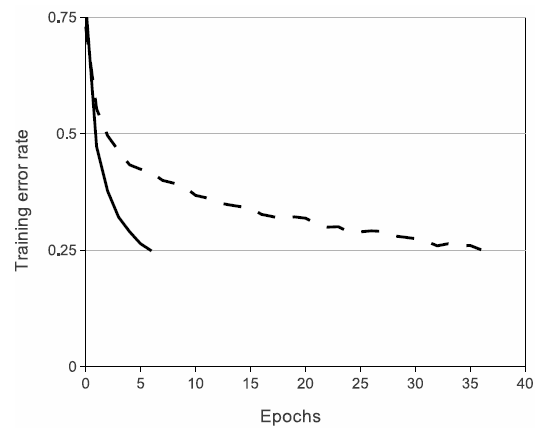
\includegraphics[width=0.49\textwidth]{relu.png}

\caption{一个使用 ReLU 的四层卷积神经网络 (实线) 在 CIFAR-10 上达到 25\% 的训练错误率, 比一个等效的使用 $tanh$ 神经元 (虚线) 的网络快 6 倍. 每个网络的学习率都是独立选择的, 以使训练尽可能快. 没有使用任何类型的正则化. 这里演示的效果的大小会随网络架构而变化, 但使用 ReLU 的网络始终比使用饱和神经元的等效网络学习得快几倍.}
\label{fig:relu}
\end{figure}

\vspace{-1mm}
\subsection{在多 GPU 上训练}
\vspace{-2ex}
单个 GTX 580 GPU 只有 3GB 内存, 这限制了可以在其上训练的网络的最大大小. 事实证明, 120 万个训练样本足以训练无法在一个 GPU 上放置的网络. 因此, 我们将网络分布在两个 GPU 上. 当前的 GPU 特别适合跨 GPU 并行化, 因为它们能够直接读取和写入彼此的内存, 而无需通过主机机器内存. 我们采用的并行化方案本质上是在每个 GPU 上放置一半的核 (或神经元), 和一个额外的技巧: GPU 仅在某些层中进行通信. 这意味着, 例如, 第 3 层的核从第 2 层的所有核映射中获取输入. 但是, 第 4 层的核仅从位于同一 GPU 上的第 3 层的那些核映射中获取输入. 选择连接模式是一个交叉验证问题, 但这使我们能够精确地调整通信量, 直到它是总体计算量的可接受比例.

最终的架构与 Cire\c{s}an 等人~\cite{cire2011} 使用的“列式” CNN 有些相似, 但我们的列式不是独立的 (见图~\ref{fig:alexnet}). 这种方案将我们的 top-1 和 top-5 错误率分别降低了 1.7\% 和 1.2\%, 与在一个 GPU 上训练的每层卷积层中只有一半的核的网络相比. 两个 GPU 的网络比一个 GPU 的网络训练时间略短\footnote{一个 GPU 的网络与两个 GPU 的网络在最终卷积层中有相同数量的核. 这是因为网络的大部分参数都在第一个全连接层中, 该层将最后一个卷积层作为输入. 所以为了让两个网络的参数数量大致相同, 我们没有减半最后一个卷积层的大小 (也没有减半后面的全连接层). 因此, 这种比较有利于一个 GPU 的网络, 因为它比两个 GPU 的网络的“一半大小”大.}.

\vspace{-1mm}
\subsection{局部响应归一化}
\vspace{-2ex}
ReLU 具有理想的特性, 即不需要进行输入归一化来防止饱和. 这意味着, 如果至少有一些训练示例将正输入提供给 ReLU, 那么该神经元将被学习. 但是, 我们发现以下局部归一化方案有助于泛化. 将由在位置 $(x,y)$ 应用核 $i$ 然后应用 ReLU 非线性计算的神经元激活值表示为 $a^i_{x,y}$, 响应规一化激活值 $b^i_{x,y}$ 由下面表达式给出
\[
b^i_{x, y} = a^i_{x, y} / \left( k + \alpha \sum^{min(N-1, i+n/2)}_{j=max(0, i-n/2)} (a^j_{x, y})^2 \right)^\beta 
\]
​
其中, 求和是在同一空间位置 $n$ 个“相邻”核映射上进行, $N$ 为层中的总核数.  核映射的排序当然是任意的, 并在训练开始之前确定. 这种响应归一化实现了一种受真实神经元中发现的类型启发的侧抑制形式, 从而创建了使用不同核计算的神经元输出之间的大激活值竞争. 常数$k$, $n$, $\alpha$ 和 $\beta$ 是超参数, 其值使用验证集确定; 我们使用 $k=2$, $n=5$, $\alpha = 10^{-4}$, 和 $\beta = 0.75$. 我们在某些层中将这种归一化应用于 ReLU 非线性之后 (见第~\ref{subsec:arch} 节).

该方案与 Jarrett 等人~\cite{jarrett2009}的局部对比度归一化方案有一定相似之处, 但我们的方案更准确地称为“亮度归一化”, 因为我们不减去平均激活值. 响应归一化分别将我们的 top-1 和 top-5 错误率降低了 1.4\% 和 1.2\%. 我们还在 CIFAR-10 数据集上验证了该方案的有效性: 一个四层 CNN 在没有归一化的情况下实现了 13\% 的测试错误率, 在有归一化的情况下实现了 11\%\footnote{由于空间限制, 我们无法详细描述这个网络, 但它由这里提供的代码和参数文件精确描述: \url{http://code.google.com/p/cuda-convnet/}}.

\vspace{-1mm}
\subsection{重叠池化}
\label{subsec:pool}
\vspace{-2ex}
卷积神经网络的池化层汇总了同一核映射中相邻神经元组的输出. 传统上, 相邻池化单元汇总的邻域不重叠 (例如, \cite{lecun2009, jarrett2009, cire2012}). 更准确地说, 池化层可以被认为是由相隔 $s$ 像素的池化单元网格组成, 每个池化单元汇总一个中心在池化单元位置的大小为 $z \times z$ 的邻域. 如果我们设置 $s = z$, 我们将获得通常在 CNN 中使用的传统局部池化. 如果我们设置 $s \le z$, 我们将获得重叠池化. 这就是我们在整个网络中使用的方法, $s = 2$ 和 $z = 3$. 与非重叠方案 $s = 2$, $z = 2$ 相比, 该方案分别将 top-1 和 top-5 错误率降低了 0.4\% 和 0.3\%. 我们在训练期间一般观察到, 具有重叠池化的模型稍微更难过拟合.

\vspace{-2mm}
\subsection{总体架构}
\label{subsec:arch}
\vspace{-2ex}
现在, 我们可以描述我们 CNN 的总体架构了. 如图~\ref{fig:alexnet} 所示, 该网络包含 8 个带权重层; 前 5 个是卷积层, 剩下 3 个是全连接层. 最后一层全连接层的输出会输入到一个 1000 路 softmax, 它会生成一个在 1000 个类别标签上的概率分布. 我们的网络最大化了多项式逻辑回归目标函数, 这等价于在预测分布下最大化训练样本中正确标签的对数概率的平均值.

卷积层 2、4 和 5 的核仅连接到位于同一 GPU 上的上一层的那些核映射 (见图~\ref{fig:alexnet}). 卷积层 3 的核连接到第 2 层的所有核映射. 全连接层中的神经元连接到上一层的所有神经元. 响应归一化层跟在第 1 和第 2 个卷积层后. 最大池化层, 如第~\ref{subsec:pool} 节描述的那种, 跟在两个响应归一化层以及第 5 个卷积层后. ReLU 非线性被应用于每个卷积层和全连接层的输出.

卷积层 1 使用 96 个大小为 $11\times 11 \times 3$ 的核对 $224 \times 224 \times 3$ 输入图像进行卷积, 步长为 4 像素 (这是核映射中相邻神经元感受野中心之间的距离). 卷积层 2 以卷积层 1 的 (响应归一化和池化后) 输出为输入, 并使用 256 个大小为 $5 \times 5 \times 48$ 的核对其进行卷积. 卷积层 3、4、5 彼此连接, 没有任何中间池化或归一化层. 卷积层 3 有 384 个大小为 $3 \times 3 \times 256$ 的核连接到卷积层 2 的 (归一化、池化后) 输出. 卷积层 4 有 384 个大小为 $3 \times 3 \times 192$ 的, 卷积层 5 有 256 个大小为 $3 \times 3 \times 192$ 的核. 全连接层每个有 4096 个神经元.

\begin{figure}
\centering
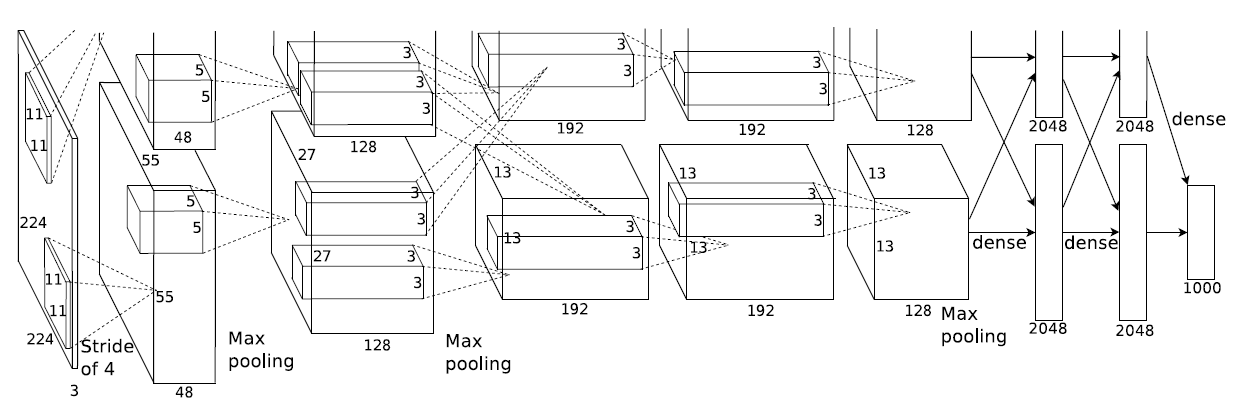
\includegraphics[width=0.98\textwidth]{alexnet.png}
\caption{一个图像卷积神经网络 (CNN) 的架构示意图, 其中明确显示了两个 GPU 之间的职责划分. 一个 GPU 运行图顶部的层部分, 而另一个 GPU 运行图底部的层部分. 两个 GPU 仅在特定层进行通信. 网络的输入是 150,528 维, 而网络剩余层的神经元数为 290,400-186,624-64,896-64,896-43,264-4096-4096-1000.}
\label{fig:alexnet}
\end{figure}

\vspace{-1mm}
\section{减少过拟合}
\label{sec:overfit}
\vspace{-2ex}
我们的神经网络架构有 6000 万个参数. 虽然 ILSVRC 的 1000 个类别使每个训练示例对图像到标签的映射施加 10 比特的约束, 但这对于学习如此多的参数却是不够的, 会导致过拟合. 下面, 我们描述了我们用来对抗过拟合的两种主要方法.

\vspace{-1mm}
\subsection{数据增强}
\label{subsec:augment}
\vspace{-2ex}
在图像数据上减少过拟合的最简单和最常用的方法是使用标签保留变换 (例如~\cite{simard2003, cire2012, cire2011}) 人工扩大数据集. 我们采用了两种不同的数据增强形式, 两种形式都允许从原始图像中生成转换后的图像, 而计算量很小, 因此不需要将转换后的图像存储在磁盘上. 在我们的实现中, 转换后的图像在 CPU 上使用 Python 代码生成, 而此时 GPU 正在训练上一批图像. 因此, 这些数据增强方案实际在计算上是没有成本的.

第一种数据增强形式是生成图像的平移和水平翻转. 我们通过从 $256 \times 256$ 图像中提取随机的 $224 \times 224$ 图像块 (以及它们的水平翻转) , 并在这些提取的图像块上训练我们的网络\footnote{这就是为什么图~\ref{fig:alexnet} 中输入图像是 $224 \times 224 \times 3$ 维}. 这会将我们的训练集大小增加了 2048 倍, 尽管由此产生的训练示例是高度相关的. 没有这种方案, 我们的网络会遭受严重的过拟合, 这将迫使我们使用更小网络. 在测试时, 网络通过提取五个 $224 \times 224$ 图像块 (四个角图像块和中心图像块) 以及它们的水平翻转 (因此总共十个图像块), 并对网络的 softmax 层在十个图像块上进行的预测进行平均来进行预测.

第二种数据增强形式是改变训练图像中 RGB 通道的强度. 具体来说, 我们对 ImageNet 训练集中的 RGB 像素值集进行 PCA. 对每个训练图像, 我们添加多个找到的主成分, 其幅值正比于相应的特征值乘以一个随机变量 (从均值为零、标准差为 0.1 的高斯分布中抽取的随机变量). 因此, 对于每个 RGB 图像像素 $I_{xy} = [I^R_{xy}, I^G_{xy}, I^B_{xy}]^T$, 我们添加以下量:
\[
[\mathbf{p}_1, \mathbf{p}_2, \mathbf{p}_3][\alpha_1\lambda_1, \alpha_2\lambda_2, \alpha_3\lambda_3]^T
\]

其中 $\mathbf{p}_i$ 和 $\lambda_i$ 分别是 $3 \times 3$ RGB 像素值协方差矩阵的第 $i$ 个特征向量和特征值, $\alpha_i$ 是上述随机变量. 每个 $\alpha_i$ 仅为特定训练图像的所有像素绘制一次, 直到该图像再次用于训练, 此时它将被重新绘制. 该方案大致捕获了自然图像的一个重要属性, 即对象标识不随照明强度和颜色的变化而变化. 该方案将 top-1 错误率降低了 1\% 以上.
\vspace{-1mm}
\subsection{Dropout}
\vspace{-2ex}
将许多不同模型的预测结合起来是一种非常成功的降低测试错误的方法~\cite{bell2007, breiman2001}, 但这对于需要几天时间来训练的大型神经网络可能很昂贵. 然而, 有一个非常有效的模型组合方法, 在训练期间只需要大约两倍的成本. 这种最近引入的技术称为“dropout”~\cite{hinton2012}, 它以 0.5 的概率随机将每个隐藏神经元的输出设置为 0. 神经网络中以这种方式的“dropped out”神经元不参与前向传递, 也不参与反向传播. 因此, 每当输入被呈现时, 神经网络都会采样一个不同的架构, 但所有这些架构都共享权重. 这种技术通过减少神经元的复杂协同适应来发挥作用, 因为神经元不能依赖特定其他神经元的存在. 因此, 它被迫学习与许多不同的随机子集一起有用的更健壮的特征. 在测试时, 我们使用所有神经元, 但将它们的输出乘以0.5, 这是一个合理的近似值, 即取指数级多个 dropout 网络产生的预测分布的几何平均值.

我们在图~\ref{fig:alexnet} 中的前两个全连接层使用了 dropout. 没有 dropout, 我们的网络会出现严重的过拟合. dropout 大致将收敛所需的迭代次数增加一倍.

\vspace{-1mm}
\section{学习细节}
\vspace{-2ex}
我们使用批量大小为 128 个示例、动量为 0.9 和权重衰减为 0.0005 的随机梯度下降训练了我们的模型. 我们发现这很小的权重衰减对于模型学习很重要. 换句话说, 权重衰减在这里不仅仅是一个正则化器: 它也降低了模型的训练误差. 权重 $w$ 的更新规则是:
\begin{align*}
v_{i+1} &:= 0.9 \cdot v_i - 0.0005 \cdot \epsilon \cdot w_i - \epsilon \cdot\left\langle  \frac{\partial L}{\partial w}|_{w_i} \right\rangle_{D_i} \\
w_{i+1} &:= w_i + v_{i+1}
\end{align*}

\begin{figure}
\centering
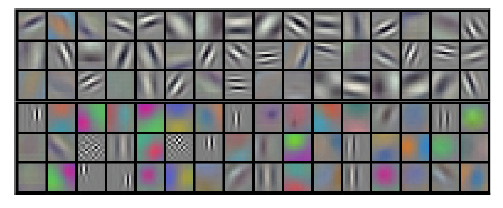
\includegraphics[width=0.49\textwidth]{kernels.png}

\caption{96 个大小为 $11 \times 11 \times 3$ 的卷积核, 由第一个卷积层在 $224 \times 224 \times 3$ 输入图像上学习. 顶部 48 个核在 GPU 1 上学习, 而底部 48 个核在 GPU 2 上学习. 细节参见第~\ref{subsec:qualitative} 节.}
\label{fig:kernels}
\end{figure}

其中, $i$ 是迭代索引, $v$ 是动量变量, $\epsilon$ 是学习率, $\langle  \frac{\partial L}{\partial w}|_{w_i} \rangle_{D_i}$ 是第 $i$ 个批次 $D_i$ 中关于 $w$ 的目标函数导数的平均值, 在 $w_i$ 处计算.

我们从均值为 0  标准差为 0.01 的正态分布中初始化每个层的权重. 我们初始化第二、四、五个卷积层以及全连接隐藏层的神经元偏置为常数 1. 这种初始化通过为 ReLU 提供正输入来加速早期学习阶段. 我们将剩余层的神经元偏置初始化为常数 0.

我们为所有层使用相同的学习率, 并在训练过程中手动调整. 我们遵循的启发式方法是, 当验证错误率不再随着当前学习率的变化而改善时, 将学习率除以 10. 学习率初始化为 0.01, 并在终止之前减少 3 次. 我们在 120 万张图像的训练集上将网络训练了大约 90 个周期, 这在两个 NVIDIA GTX 580 3GB 显卡上花了五到六天.

\vspace{-1mm}
\section{结果}
\label{sec:result}
\vspace{-2ex}
我们在 ILSVRC-2010 上的结果总结在表~\ref{tab:ilsvrc2010} 中. 我们的网络实现了 \textbf{37.5\%} 和 \textbf{17.0\%} 的 top-1 和 top-5 测试集错误率\footnote{没有使用如第~\ref{subsec:augment} 节所述的对10个图像块的预测进行平均的方法, 错误率分别为 39.0\% 和 18.3\%.}. ILSVRC-2010 竞赛期间取得的最佳性能为 47.1\% 和 28.2\%, 使用的方法是平均从六个在不同特征上训练的稀疏编码模型生成的预测~\cite{berg2010}, 在这之后, 最佳的已发布结果为 45.7\% 和 25.7\%, 使用的方法是平均两个分类器的预测, 这些分类器是使用由两种类型的密集采样特征计算的 Fisher 向量 (FVs) 训练的~\cite{sanchez2011}.

\begin{table}
\centering
\begin{tabular}{|c|c|c|}
  \hline
  \textbf{Model} & \textbf{Top-1} & \textbf{Top-5} \\
  \hline
  \hline
  \emph{Sparse coding~\cite{berg2010}} & \emph{47.1\%} & \emph{28.2\%} \\
  \hline
  \emph{SIFT + FVs~\cite{sanchez2011}} & \emph{45.7\%} & \emph{25.7\%} \\
  \hline
  CNN & \textbf{37.5\%} & \textbf{17.0\%} \\
  \hline
\end{tabular}

\caption{ILSVRC-2010 测试集上结果的比较. \emph{斜体}表示由其他人取得的最佳结果.}
\label{tab:ilsvrc2010}
\end{table}

我们也将我们的模型输入了 ILSVRC-2012 竞赛, 并在表~\ref{tab:ilsvrc2012} 中报告了我们的结果. 由于 ILSVRC-2012 测试集标签没有公开发布, 我们不能为所有我们尝试过的模型报告测试错误率. 在本段的其余部分中, 我们将验证错误率和测试错误率互换使用, 因为在我们的经验中, 它们不会相差超过 0.1\% (见表~\ref{tab:ilsvrc2012}). 本文描述的 CNN 实现了 18.2\% 的 top-5 错误率. 将五个类似的 CNN 的预测平均会给出 16.4\% 的错误率. 训练一个 CNN, 在最后的池化层之后添加一个额外的卷积层 6, 分类完整 ImageNet Fall 2011 发布版 (1500 万张图像, 22,000 个类别), 然后在 ILSVRC-2012 上对其进行“微调”, 会给出 16.6\% 的错误率. 将两个在完整 Fall 2011 发布版上预训练的 CNN 与前面提到的五个 CNN 的预测平均会给出 \textbf{15.3\%} 的错误率. 竞赛的第二名的使用一种平均了几种在不同类型的密集采样特征上训练的 FV 分类器的预测的方法, 实现了 26.2\% 的错误率.

\begin{table}
\centering
\begin{tabular}{|c|c|c|c|}
  \hline
  \textbf{Model} & \textbf{Top-1 (val)} & \textbf{Top-5 (val)} & \textbf{Top-5 (test)}\\
  \hline
  \hline
  \emph{SIFT + FVs~\cite{deng2012}} & -- & -- & \emph{26.2\%} \\
  \hline
  1 CNN & 40.7\% & 18.2\% & --\\
  \hline
  5 CNNs & 38.1\% & 16.4\% & \textbf{16.4\%}\\
  \hline
  1 CNN* & 39.0\% & 16.6\% & --\\
  \hline
  7 CNN* & 36.7\% & 15.4\% & \textbf{15.3\%} \\
  \hline
\end{tabular}

\caption{ILSVRC-2012 验证集和测试集上错误率的比较. \emph{斜体}表示由其他人取得的最佳结果. 带星号 (*) 的模型使用了“预训练”, 分类完整的 ImageNet 2011 Fall 发布版. 细节参见第~\ref{sec:result} 节.}
\label{tab:ilsvrc2012}
\end{table}

最后, 我们还报告了我们在 ImageNet Fall 2009 版上的错误率, 该版有 10,184 个类别和 890 万张图像. 在这个数据集上, 我们遵循文献中使用一半的图像进行训练和一半的图像进行测试的惯例. 由于没有规定的测试集, 我们的拆分必然不同于先前作者使用的拆分, 但这不会显著影响结果. 我们在该数据集上的 top-1 和 top-5 错误率为 \textbf{67.4\%} 和 \textbf{40.9\%}, 由上面描述的网络实现, 但在最后的池化层后添加了一个额外的卷积层 6. 该数据集上已发布的最佳结果为 78.1\% 和 60.9\%~\cite{mensink2012}.

\vspace{-1mm}
\subsection{定性评估}
\label{subsec:qualitative}
\vspace{-2ex}
图~\ref{fig:kernels} 显示了网络的两个数据连接层学习到的卷积核. 网络已经学习了各种频率和方向选择性核, 以及各种色块. 注意两个 GPU 所表现出的特化, 这源于第~\ref{subsec:arch} 节中描述的受限连接性. GPU 1 上的核在很大程度上是颜色无关的, 而 GPU 2 上的核在很大程度上是颜色特定的. 这种特化在每次运行时都会发生, 并且与任何特定的随机权重初始化无关 (除了 GPU 的重新编号).

\begin{figure}
\centering
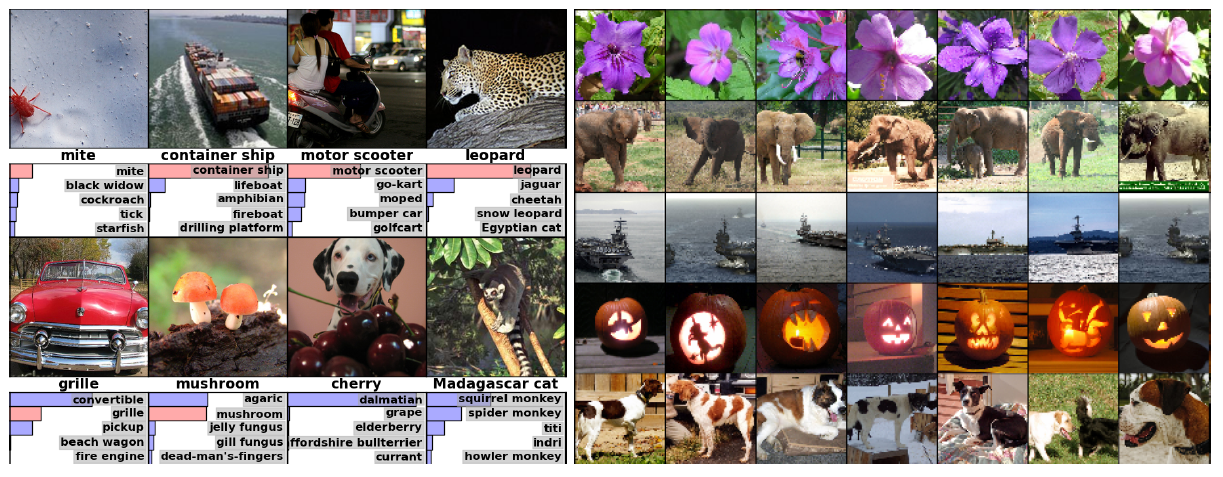
\includegraphics[width=0.98\textwidth]{qualitative.png}

\caption{(左) 八张 ILSVRC-2010 测试图像和我们的模型认为最可能的五个标签. 每个图像下方写着正确的标签, 如果正确的标签在前五名中, 则还会显示分配给正确标签的概率 (用红色条表示). (右) 第一列是五张 ILSVRC-2010 测试图像. 其余列显示了在最后一个隐藏层生成的特征向量与测试图像的特征向量最小欧几里得距离的六个训练图像.}
\label{fig:qualitative}
\end{figure}

在图~\ref{fig:qualitative} 的左面板中, 我们通过计算网络在 8 张测试图像上的 top-5 预测来定性地评估网络所学到的内容. 注意, 即使是偏心的物体, 例如左上角的螨虫, 也可以被网络识别. 大多数 top-5 标签看起来都很合理. 例如, 只有其他类型的猫被认为是豹子的可行标签. 在某些情况下 (格栅、樱桃), 照片的预期焦点存在不确定性.

另一种探究网络视觉知识的方法是考虑图像在最后一个 4096 维隐藏层中产生的特征激活. 如果两个图像产生的特征激活向量具有小欧几里得间隔, 我们可以说神经网络的更高层次认为它们是相似的. 图~\ref{fig:qualitative} 显示了测试集的五张图像以及根据该度量标准最相似的六张训练集图像. 注意, 在像素级别上, 检索到的训练图像通常不会与第一列的查询图像在 L2 中接近. 例如, 检索到的狗和大象以多种姿势出现. 我们在补充材料中提供了更多测试图像的结果.

计算两个 4096 维实值向量之间的欧几里得距离来计算相似性效率低下, 但可以通过训练一个自动编码器来压缩这些向量为短二进制代码来提高效率. 这应该比将自动编码器应用于原始像素~\cite{krizhevsky2011} 产生一个更好的图像检索方法, 因为它不使用图像标签, 因此倾向于检索具有相似边缘模式的图像, 无论它们是否具有语义相似性.

\vspace{-2mm}
\section{讨论}
\vspace{-3ex}

我们的结果表明, 一个大型的深度卷积神经网络能够使用纯监督学习在极具挑战性的数据集上实现破纪录的结果. 值得注意的是, 如果删除单个卷积层, 我们的网络性能会下降. 例如, 移除任何中间层会导致网络的 top-1 性能损失约 2\%. 因此, 深度对于实现我们的结果确实很重要.

为了简化我们的实验, 我们没有使用任何无监督的预训练, 即使我们认为它会有所帮助, 特别是如果我们获得足够的计算能力来显著增加网络的大小而没有获得相应增加的标记数据量. 到目前为止, 我们的结果已经得到了改善, 因为我们已经使我们的网络更大而且训练的时间更长, 但是为了匹配人类视觉系统的 infero-temporal 路径, 我们还有很多数量级的工作要做. 最终, 我们希望在视频序列上使用非常大且深的卷积网络, 其中时间结构提供了非常有用的信息, 而这些信息在静态图像中缺失或不太明显.
%-------------------------------------------------------------------------


%{\small
%\bibliographystyle{ieee}
%
%\begin{thebibliography}
%
%
%
%\bibitem{Todorovic_ECCV2010}
%N. Payet and S. Todorovic, From a Set of Shape to Object Discoverty, In {\em ECCV}, 2010.
%
%
%
%
%\end{thebibliography}
%}


\small
\bibliographystyle{ieee}
\begin{thebibliography}{99}

\bibitem{bell2007} % 1
R.M. Bell and Y. Koren. Lessons from the netflix prize challenge. {\em ACM SIGKDD Explorations Newsletter}, 9(2):75–79, 2007.
\vspace{-1mm}

\bibitem{berg2010} % 2
A. Berg, J. Deng, and L. Fei-Fei. Large scale visual recognition challenge 2010. \url{www.imagenet.org/challenges}. 2010.
\vspace{-1mm}

\bibitem{breiman2001} % 3
L. Breiman. Random forests. {\em Machine learning}, 45(1):5–32, 2001.
\vspace{-1mm}

\bibitem{cire2012} % 4
D. Cire\c{s}an, U. Meier, and J. Schmidhuber. Multi-column deep neural networks for image classification.
{\em Arxiv preprint arXiv:1202.2745}, 2012.
\vspace{-1mm}

\bibitem{cire2011} % 5
D.C. Cire\c{s}an, U. Meier, J. Masci, L.M. Gambardella, and J. Schmidhuber. High-performance neural
networks for visual object classification. {\em Arxiv preprint arXiv:1102.0183}, 2011.
%\vspace{-1mm}

\bibitem{deng2009} % 6
J. Deng, W. Dong, R. Socher, L.-J. Li, K. Li, and L. Fei-Fei. ImageNet: A Large-Scale Hierarchical
Image Database. In {\em CVPR09}, 2009.
\vspace{-1mm}

\bibitem{deng2012} % 7
J. Deng, A. Berg, S. Satheesh, H. Su, A. Khosla, and L. Fei-Fei. {\em ILSVRC-2012}, 2012. URL
\url{http://www.image-net.org/challenges/LSVRC/2012/}.
\vspace{-1mm}

\bibitem{feifei2007} % 8
L. Fei-Fei, R. Fergus, and P. Perona. Learning generative visual models from few training examples: An
incremental bayesian approach tested on 101 object categories. {\em Computer Vision and Image Understanding},
106(1):59–70, 2007.
\vspace{-1mm}

\bibitem{griffin2007} % 9
G. Griffin, A. Holub, and P. Perona. Caltech-256 object category dataset. Technical Report 7694, California
Institute of Technology, 2007. URL \url{http://authors.library.caltech.edu/7694}.
\vspace{-1mm}

\bibitem{hinton2012} % 10
G.E. Hinton, N. Srivastava, A. Krizhevsky, I. Sutskever, and R.R. Salakhutdinov. Improving neural networks
by preventing co-adaptation of feature detectors. {\em arXiv preprint arXiv:1207.0580}, 2012.
\vspace{-1mm}

\bibitem{jarrett2009} % 11
K. Jarrett, K. Kavukcuoglu, M. A. Ranzato, and Y. LeCun. What is the best multi-stage architecture for
object recognition? In {\em International Conference on Computer Vision}, pages 2146–2153. IEEE, 2009.
\vspace{-1mm}

\bibitem{krizhevsky2009} % 12
A. Krizhevsky. Learning multiple layers of features from tiny images. Master's thesis, Department of
Computer Science, University of Toronto, 2009.
\vspace{-1mm}

\bibitem{krizhevsky2010} % 13
A. Krizhevsky. Convolutional deep belief networks on cifar-10. {\em Unpublished manuscript}, 2010.
\vspace{-1mm}

\bibitem{krizhevsky2011} % 14
A. Krizhevsky and G.E. Hinton. Using very deep autoencoders for content-based image retrieval. In
{\em ESANN}, 2011.
\vspace{-1mm}

\bibitem{lecun1990} % 15
Y. LeCun, B. Boser, J.S. Denker, D. Henderson, R.E. Howard, W. Hubbard, L.D. Jackel, et al. Handwritten
digit recognition with a back-propagation network. In {\em Advances in neural information processing
systems}, 1990.
\vspace{-1mm}

\bibitem{lecun2004} % 16
Y. LeCun, F.J. Huang, and L. Bottou. Learning methods for generic object recognition with invariance to
pose and lighting. In {\em Computer Vision and Pattern Recognition, 2004. CVPR 2004. Proceedings of the
2004 IEEE Computer Society Conference on}, volume 2, pages II–97. IEEE, 2004
\vspace{-1mm}

\bibitem{lecun2009} % 17
Y. LeCun, K. Kavukcuoglu, and C. Farabet. Convolutional networks and applications in vision. In
{\em Circuits and Systems (ISCAS), Proceedings of 2010 IEEE International Symposium on}, pages 253–256.
IEEE, 2010.
\vspace{-1mm}

\bibitem{lee2009} % 18
H. Lee, R. Grosse, R. Ranganath, and A.Y. Ng. Convolutional deep belief networks for scalable unsupervised
learning of hierarchical representations. In {\em Proceedings of the 26th Annual International Conference
on Machine Learning}, pages 609–616. ACM, 2009.
\vspace{-1mm}

\bibitem{mensink2012} % 19
T. Mensink, J. Verbeek, F. Perronnin, and G. Csurka. Metric Learning for Large Scale Image Classification:
Generalizing to New Classes at Near-Zero Cost. In {\em ECCV - European Conference on Computer
Vision}, Florence, Italy, October 2012.
\vspace{-1mm}

\bibitem{nair2010} % 20
V. Nair and G. E. Hinton. Rectified linear units improve restricted boltzmann machines. In {\em Proc. 27th
International Conference on Machine Learning}, 2010.
\vspace{-1mm}

\bibitem{pinto2008} % 21
N. Pinto, D.D. Cox, and J.J. DiCarlo. Why is real-world visual object recognition hard? {\em PLoS computational
biology}, 4(1):e27, 2008.
\vspace{-1mm}

\bibitem{pinto2009} % 22
N. Pinto, D. Doukhan, J.J. DiCarlo, and D.D. Cox. A high-throughput screening approach to discovering
good forms of biologically inspired visual representation. {\em PLoS computational biology}, 5(11):e1000579,
2009.
\vspace{-1mm}

\bibitem{russell2008} % 23
B.C. Russell, A. Torralba, K.P. Murphy, and W.T. Freeman. Labelme: a database and web-based tool for
image annotation. {\em International journal of computer vision}, 77(1):157–173, 2008.
\vspace{-1mm}

\bibitem{sanchez2011} % 24
J. S\'{a}nchez and F. Perronnin. High-dimensional signature compression for large-scale image classification.
In {\em Computer Vision and Pattern Recognition (CVPR), 2011 IEEE Conference on}, pages 1665–1672. IEEE,
2011.
\vspace{-1mm}

\bibitem{simard2003} % 25
P.Y. Simard, D. Steinkraus, and J.C. Platt. Best practices for convolutional neural networks applied to
visual document analysis. In {\em Proceedings of the Seventh International Conference on Document Analysis
and Recognition}, volume 2, pages 958–962, 2003.
\vspace{-1mm}

\bibitem{turaga2010} % 26
S.C. Turaga, J.F. Murray, V. Jain, F. Roth, M. Helmstaedter, K. Briggman,W. Denk, and H.S. Seung. Convolutional
networks can learn to generate affinity graphs for image segmentation. {\em Neural Computation},
22(2):511–538, 2010.
\vspace{-1mm}


\end{thebibliography}


\end{document}
